\section{Methodology}
In this section, we outline the methodology employed to gather, process, and annotate the data for our study. We begin by detailing the sources of our multimodal video data and personality labels, focusing on how we efficiently align subtitles with original scripts to ensure accurate temporal and character associations. And we also present our annotation process, explaining how we leverage the ChatGPT API to automatically annotate social and emotional relations among characters within the text data. 
\subsection{Source of Data}
Our data source contains mainly two parts, the multimodal video data and personality labels. For video data, we include 14 different genres of TV series and movies via an open-source website\footnote[1]{https://yts.mx/}, and for the scripts and subtitles, we also find other open-source websites\footnote[2]{https://www.simplyscripts.com/}\footnote[3]{https://subscene.com/} for research offering the free scripts and subtitles of many famous movie and television programs. Considering the insufficient labeling method of existing works, we collect the personality annotations from personality database website as well as the voting distribution and align them to correctly scripts. 
\subsection{Data Alignment Process}
As subtitle contain temporal information and original scripts associate utterances with characters, we are supposed to align them properly as efficient as possible. However, most of the existing multimodal datasets annotate the timestamps manually with taking up a great deal of time. There are also some works which utilize different automatic tools to align the utterances with their corresponding information. For instance, \cite{lian2024merbench} use an Automatic Sound Recognition (ASR) tool called Gentle\footnote[4]{https://github.com/lowerquality/gentle} to get the timestamps for the utterances. To streamline the process of aligning dialogue utterances with their respective timestamps and speakers from subtitles, we propose an efficient method leveraging a fuzzy matching algorithm. 
Following successful alignment, we proceed to segment the video content into distinct scenes according to the timestamps. Besides, we use FFmpeg\footnote[5]{https://ffmpeg.org/} to extract the audio track from the video clips and output it as a \textit{.mp3} file.


\begin{figure}[ht]
    \small
    \centering 	 	 	 	
    \includegraphics[width=\linewidth, trim= 0 10 0 10, clip]{images/raw_data.pdf}
	\caption{Process of data alignment}
    \label{fig:alig}
\end{figure}

\subsection{Annotation Process}

We developed a process to automatically annotate social and emotional relationships among characters using the ChatGPT API, specifically the \textit{gpt-3.5-turbo-1106} model, which is suited for processing text data. After preprocessing the text and dividing it into scenes, we designed prompts (Fig \ref{fig:prompt}) for ChatGPT to identify social and emotional relationships in each scene. A challenge arose in representing unidirectional affectionate relationships, where one character (A) likes another (B) but the feeling is not mutual. While social relationships are straightforward, emotional relationships require a method to capture this directionality. We addressed this by interpreting the relative position of characters in the tuple: for instance, "A and B (family, fondness)" indicates that A has positive feelings towards B, whereas "B and A (family, fondness)" indicates the opposite. This method effectively captures and represents the directionality of emotional relationships.

\begin{figure}[ht]
	\centering
	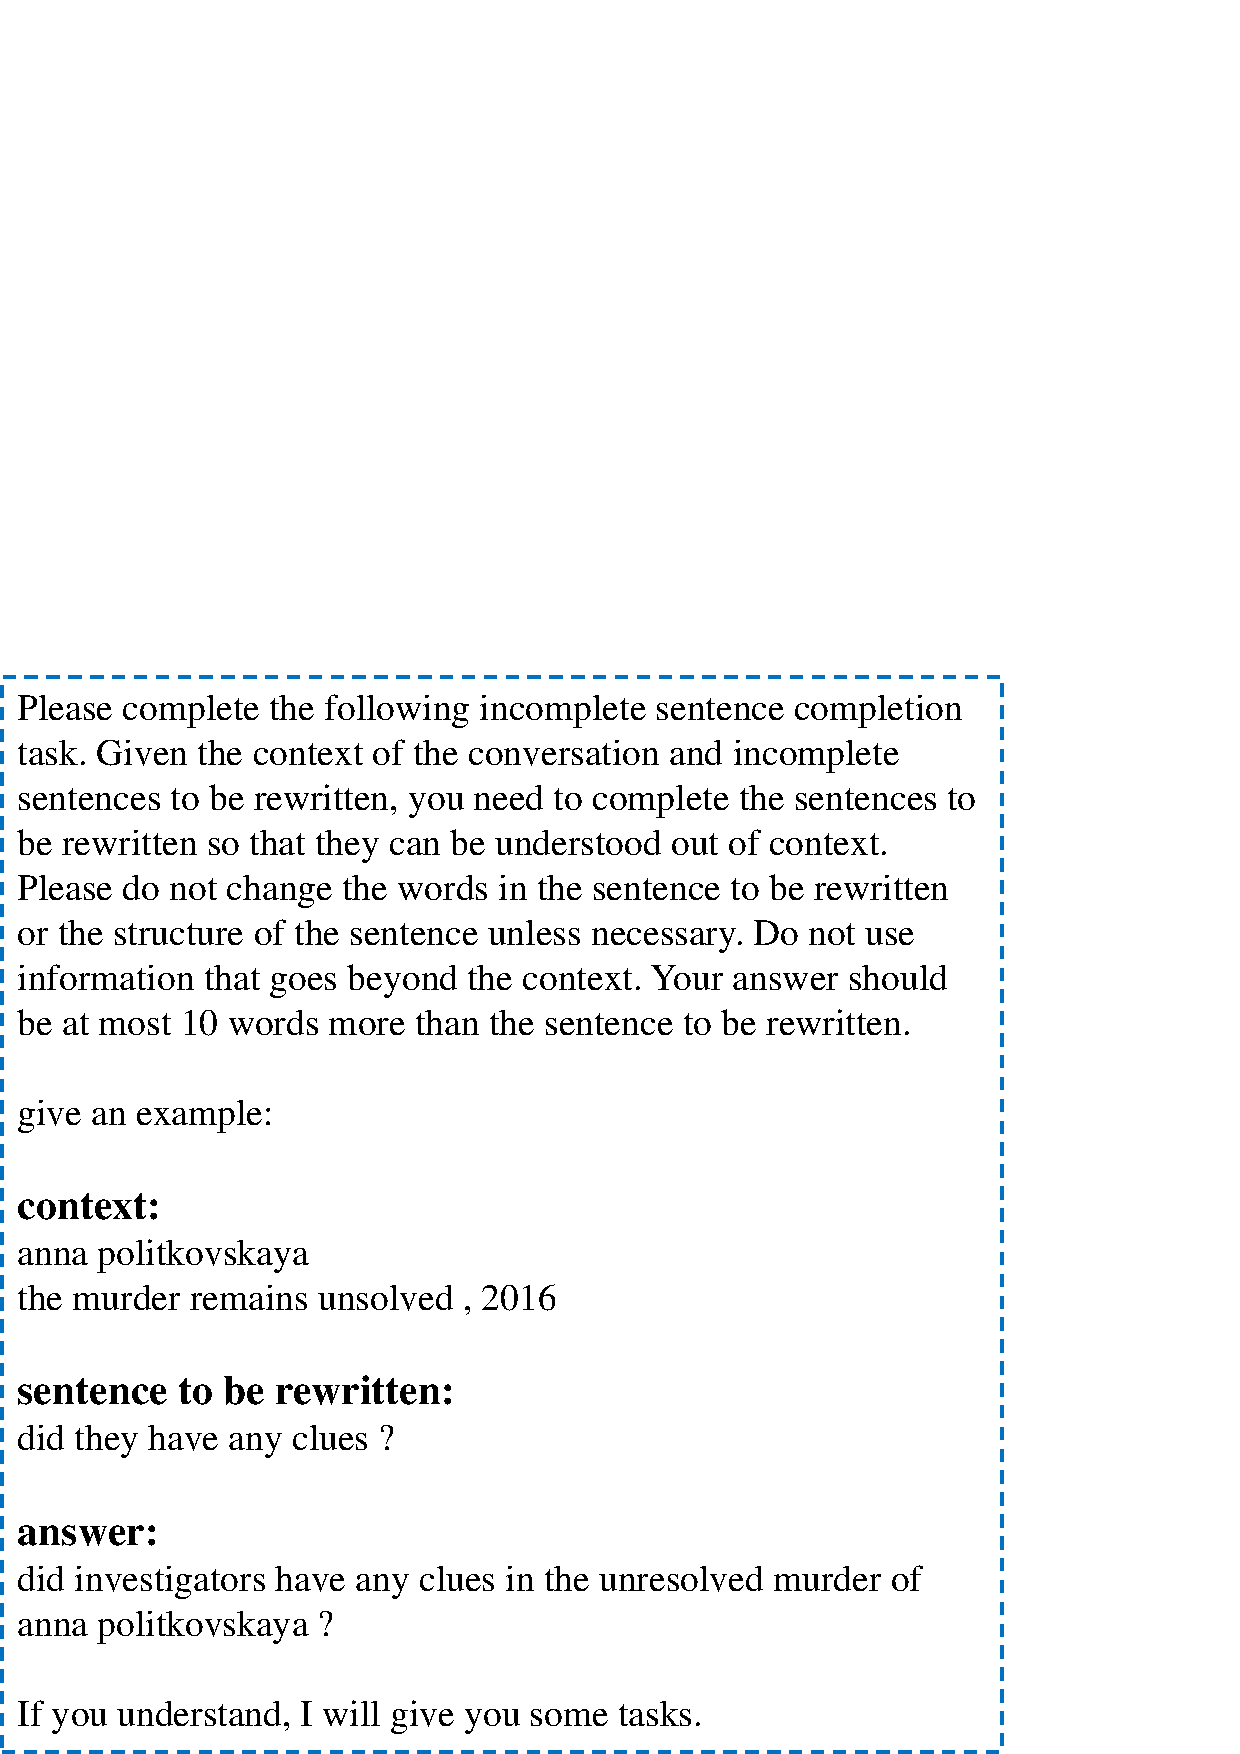
\includegraphics[width=\linewidth]{images/prompt.pdf}
	\caption{Prompt design for relations annotation}
	\label{fig:prompt}
\end{figure}

